\documentclass[a4paper,12pt]{article}

% Packages
\usepackage[utf8x]{inputenc}
\usepackage{amsmath}
\usepackage{amssymb}
\usepackage{graphicx}
\usepackage{hyperref}
\usepackage{geometry}
\usepackage{bookmark}
\usepackage{fancyhdr}
\usepackage{physics}
\usepackage{unicode-math}
\usepackage{lmodern}
\usepackage{pdfpages}
\usepackage{simpler-wick}
\usepackage{unicode-math}
\usepackage{caption}

% Page geometry
\geometry{margin=1in}

% Header and Footer
\pagestyle{fancy}
\fancyhf{}
\fancyhead[L]{First midterm FYS4480}
\fancyhead[R]{FYS4480}
\fancyfoot[C]{\thepage}

% Document information
\title{Midterm 1}
\author{Hishem Kløvnes}
\date{\today}

\begin{document}

\maketitle

\section{Quantum mechanics for many-particle systems}
Note: Link to codes and the diagrams are placed at the end of the document.\\
\subsection*{a)}
We start with the helium atom and define our single particle Hilbert space to consist of the single-particle orbits $1s$, $2s$ and $3s$, with their corresponding spin degenracies.\\
Ansatz for the ground state $\ket{c} = \ket{Φ_0}$ in second quantization:
\[
\ket{c} = a_{1s,{\uparrow}}^\dagger a_{1s,{\downarrow}}^\dagger \ket{0}
\]

\[
\begin{matrix}
    n & m_s &  \\
    1 & +\frac{1}{2} & \uparrow \\
    1 & -\frac{1}{2} & \downarrow \\
    2 & +\frac{1}{2} & \uparrow \\
    2 & -\frac{1}{2} & \downarrow \\
    3 & +\frac{1}{2} & \uparrow \\
    3 & -\frac{1}{2} & \downarrow \\
    
\end{matrix}
\]

Now we need to contruct all possible one-particle-one-hole excitations from the ground state, $ \ket{ Φ_i^a}$. $i$ are levels below the Fermi level and $a$ refers to particle states. 
\begin{align*}
\ket{Φ_{1s σ }^{2s σ  }} &= a_{2s σ }^\dagger a_{1s σ } \ket{Φ_0} \\
\ket{Φ_{1s σ }^{3s σ  }} &= a_{3s σ }^\dagger a_{1s σ } \ket{Φ_0} \\
\end{align*}
Where $σ $ refers to the spin of the electron $σ ∈ \{↑ , ↓\} = \{+\frac{1}{2 }, -\frac{1}{2}\}$.\\
And for the two-particle-two-hole excitations, $ \ket{ Φ_{ij}^{ab}}$:
\begin{align*}
    \ket{Φ_{1s σ 1s -σ }^{2s σ 2s -σ }} &= a_{2s σ }^\dagger a_{2s -σ }^\dagger a_{1s σ } a_{1s -σ } \ket{Φ_0} \\
    \ket{Φ_{1s σ 1s -σ }^{3s σ 3s -σ }} &= a_{3s σ }^\dagger a_{3s -σ }^\dagger a_{1s σ } a_{1s -σ } \ket{Φ_0} \\
\end{align*}
With the same values for $σ $ as above, and keeping the Pauli principle in mind.\\

\subsection*{b)}
The general form of the second-quantized Hamiltonian for a system with two-body interactions is:
$$\hat{H} = \sum_{αβ} \bra{α} \hat{h}_0 \ket{β} a_α^\dagger a_β + \frac{1}{4} \sum_{α β γ δ } \bra{α β } \frac{1}{r} \ket{γδ}_{AS} a_α^\dagger a_q^\dagger a_γ a_δ$$
Applying the Hamiltonian to the ground state $\ket{Φ_0}$:
$$E[\Phi_0] = \bra{Φ_0} \hat{H} \ket{Φ_0}$$ 
$$E[\Phi_0] =  \sum_{αβ} \bra{α} \hat{h}_0 \ket{β}\bra{Φ_0}  a_α^\dagger a_β \ket{Φ_0} + \frac{1}{4}  \sum_{α β γ δ } \bra{α β } \frac{1}{r} \ket{γδ}_{AS}\bra{Φ_0} a_α^\dagger a_β^\dagger a_γ a_δ \ket{Φ_0}$$
We can take the one body term first:
$$\sum_{αβ} \bra{α} \hat{h}_0 \ket{β}\bra{Φ_0}  a_α^\dagger a_β \ket{Φ_0} =\sum_{αβ} \bra{α} \hat{h}_0 \ket{β}\bra{c} a_α^\dagger a_β \ket{0}$$
$$ = ∑_{ij}^{}  \bra{i} \hat{h}_0 \ket{ j} δ_{ij} = ∑_{i} \bra{i} \hat{h}_0 \ket{ i}$$ 
Which we got from contracting the creation and annihilation operators.\\
For the two body term:
$$\bra{Φ_0} \hat{H}_I \ket{Φ_0} = \frac{1}{4} ∑_{ij}  \bra{α β } V\ket{γδ}_{AS} \bra{c} a_α^\dagger a_β^\dagger a_γ a_δ \ket{c}$$
$$ = \frac{1}{4} ∑_{ij}  \bra{α β } V\ket{γδ}_{AS} \bra{0} a_j a_i a_α ^{†} a_β ^{†} a_γ a_δ a_i ^{†} a_j ^{†} \ket{0}$$
Now we can take a look at the contractions:
$$
\bra{0}
\wick{
  \c2 a_j \c1 a_i \c1 a_α^{†} \c2 a_β^{†} \c2 a_γ \c1 a_δ \c1 a_i^{†} \c2 a_j^{†}
  }
  \ket{0} = δ_{j β}δ_{i α}δ_{γj}δ_{δ i}
$$
$$
\bra{0}
\wick{
  \c2a_j \c1a_i \c1a_α^{†} \c2a_β^{†} \c2a_γ \c1a_δ \c2a_i^{†} \c1a_j^{†}
  }
  \ket{0} =- δ_{j β}δ_{i α}δ_{γi}δ_{δ j}
$$
$$
\bra{0}
\wick{
  \c2a_j \c1a_i \c2a_α^{†} \c1a_β^{†} \c2a_γ \c1a_δ \c2a_i^{†} \c1a_j^{†}
  }
  \ket{0} = δ_{j α}δ_{i β}δ_{γi}δ_{δ j}
$$
$$
\bra{0}
\wick{
  \c2a_j \c1a_i \c2a_α^{†} \c1a_β^{†} \c2a_γ \c1a_δ \c1a_i^{†} \c2a_j^{†}
  }
  \ket{0} = -δ_{jα}δ_{iβ}δ_{γi}δ_{δ j}
$$
In chronological order, we get the terms:
$$ \bra{ij} \hat{V} \ket{ij}_{AS}, -\bra{ij} \hat{V} \ket{ji}_{AS}, \bra{ji} \hat{ V} \ket{ji}_{AS}, -  \bra{ ji} \hat{V} \ket{ij}_{AS} $$
And since $  \bra{ij} \hat{ V} \ket{ij} = - \bra{ ji} \hat{V} \ket{ji}$, we can simplify the expression to:
$$ \bra{ c} \hat{H}_I \ket{ c} = \frac{1}{2} ∑_{ij} \bra{ ij} V \ket{ij}_{AS} = \frac{1}{2} ∑_{ij}^{} \bra{ ij} \frac{1}{r_{ij}} \ket{ij} - \bra{ij} \frac{1}{r_{ij}} \ket{ji} $$
And so the full energy of the system is:
$$ E[\Phi_0] = ∑_{i} \bra{ i} \hat{h}_0 \ket{ i} + \frac{1}{2} ∑_{ij} \left[ \bra{ ij} V \ket{ij} - \bra{ ij} V \ket{ji} \right] $$
The energy of from the one-body term is:
$$ \bra{ Φ_0} \hat{H}_0  \ket{Φ_0} = ∑_{i} \bra{ i} \hat{h}_0 \ket{ i} = 2\left( -\frac{Z^2}{2} \right)  = -Z^2 $$
The energy from the two-body term is:
$$ \bra{ Φ_0} \hat{H}_I  \ket{Φ_0} = \frac{1}{2} ∑_{ij} \left[ \bra{ ij} V \ket{ij} - \bra{ ij} V \ket{ji} \right] = 2 * \frac{1}{2} * \frac{5Z}{8} = \frac{5Z}{8} $$
The helium atom has $Z=2$, and so the total energy of the system is:
$$ E[\Phi_0] = -4 + \frac{5}{4} = -\frac{11}{4}=74.8eV$$

\subsection*{c)}
For this exercise, we are going to explore the one-particle-one-hole excitations $  \bra{c} \hat{H} \ket{Φ_i^a} $ and $ \bra{ Φ_i ^a} \hat{ H} \ket{ Φ_j^b}$.\\
For the more complicated systems, we can split the Hamiltionan:
$$ \hat{H} = \mathcal{E}_0^{ref} + \hat{F}_N + \hat{ V}_N$$
Where $\mathcal{E}_0^{ref}$ is the reference energy, or the ground state energy of the system, $\hat{F}_N$ is the normal-ordered one-body part of the Hamiltonian and $\hat{V}_N$ is the normal-ordered two-body part of the Hamiltonian.\\
$$ \hat{ F}_N = ∑_{pq} \bra{p} \hat{f} \ket{q} a_p ^{†} a_q, \quad \bra{ p} \hat{ f} \ket{ q} = \bra{ p} \hat{h}_0 \ket{ q} ∑_{i} \bra{p i} \hat{ V} \ket{ qi}_{AS} $$
$$ \hat{ V}_N = \frac{1}{4} ∑_{pqrs} \bra{pq} \hat{v} \ket{rs} a_p ^{†} a_q ^{†} a_s a_r$$
Now we can start with $  \bra{c} \hat{H} \ket{Φ_i^a} $:
$$ \bra{c} \mathcal{E}_0^{ref} \ket{Φ_i^a}  = 0$$
$$ \bra{ c} \hat{F}_N \ket{Φ_i^a} = ∑_{pq} \bra{p} \hat{f} \ket{q} \bra{c} a_p ^{†} a_q \ket{Φ_i^a}$$
Here we can take a look at the contractions:
$$ \bra{ c} a_p ^{†} a_q a_a^{†} a_i \ket{c}$$
$$
\bra{0}
\wick{
  \c2a_p \c1a_q \c1a_a^{†} \c2a_i^{†}
  }
\ket{0} = δ_{p i}δ_{q a}
$$
Then we get:
$$ \bra{ c} \hat{F}_N \ket{Φ_i^a} = \bra{i} \hat{f} \ket{a} = \bra{ i} \hat{h}_0 \ket{ a} + ∑_{j} \bra{ij} \hat{V} \ket{aj}$$
For the two-body term:
$$ \bra{ c} \hat{V}_N \ket{Φ_i^a} = \frac{1}{4} ∑_{pqrs} \bra{pq} \hat{v} \ket{rs} \bra{c} a_p ^{†} a_q ^{†} a_s a_r \ket{Φ_i^a} = 0$$
This is because to perform contractions, we would have to contract whithin the normal ordered operator, which would result in zero.\\
Therefor, the total expression for $  \bra{c} \hat{H} \ket{Φ_i^a} $ is:
$$ \bra{c} \hat{H} \ket{Φ_i^a} = \bra{ i} \hat{h}_0 \ket{ a} + ∑_{j} \bra{ij} \hat{V} \ket{aj}$$
Now we can move on to $ \bra{ Φ_i ^a} \hat{ H} \ket{ Φ_j^b}$:
$$ \bra{ Φ_i ^a} \mathcal{E}_0^{ref} \ket{ Φ_j^b} = \mathcal{E}_0^{ref} δ_{ij}δ_{ab}$$
$$ \bra{ Φ_i ^a} \hat{F}_N \ket{ Φ_j^b} = ∑_{pq} \bra{p} \hat{f} \ket{q} \bra{ Φ_i ^a} a_p ^{†} a_q \ket{ Φ_j^b}$$
$$
\bra{ Φ_i ^a} a_p ^{†} a_q \ket{ Φ_j^b} = \bra{c} a_i^{†} a_a a_p ^{†} a_q  a_b ^{†} a_j \ket{c} 
$$
$$
\bra{c}
\wick{
  \c2a_i^{†}\c1a_a\c1a_p^{†}\c1a_q\c1a_b^{†}\c2a_j
  }
\ket{c} = δ_{ij}δ_{ap}δ_{qb}nverged in 15 iterations
Final single-particle energies: [-0.888475   -0.888475    0.03942215  0.03942215  0.43951618  0.43951618]
Final ground state energy: -2.831096086785042
In electron volts: -77.03804842059728 eV
$$
$$
\bra{ c}
\wick{
  \c1 a_i^{†} \c2 a_a \c1 a_p^{†} \c3 a_q \c2 a_b^{†} \c3 a_j
  }
\ket{c} = -δ_{iq}δ_{ab}δ_{qj}
$$
Then we get:
$$ \bra{ Φ_i ^a} \hat{F}_N \ket{ Φ_j^b} = \bra{ a} \hat{f} \ket{ b} δ_{ij} - \bra{ j} \hat{f} \ket{ i} δ_{ab}$$
And lastly for the two-body term:
$$ \bra{ Φ_i ^a} \hat{V}_N \ket{ Φ_j^b} = \frac{1}{4} ∑_{pqrs} \bra{pq} \hat{v} \ket{rs} \bra{ Φ_i ^a} a_p ^{†} a_q ^{†} a_s a_r \ket{ Φ_j^b}$$
$$
\bra{ Φ_i ^a} a_p ^{†} a_q ^{†} a_s a_r \ket{ Φ_j^b} = \bra{c} a_i^{†} a_a a_p ^{†} a_q ^{†} a_s a_r a_b ^{†} a_j \ket{c}$$
Now we can take a look at the contractions again:
$$
\bra{c}
\wick{
  \c2a_i^{†} \c1a_a \c1a_p^{†} \c3a_q^{†} \c2a_s \c1a_r \c1a_b^{†} \c3a_j
  }
\ket{c} = -δ_{ap}δ_{is}δ_{qj}δ_{br}
$$
$$nverged in 15 iterations
Final single-particle energies: [-0.888475   -0.888475    0.03942215  0.03942215  0.43951618  0.43951618]
Final ground state energy: -2.831096086785042
In electron volts: -77.03804842059728 eV
\bra{c}
\wick{
  \c2a_i^{†} \c1a_a \c1a_p^{†} \c1a_q^{†} \c3a_s \c2a_r \c3a_b^{†} \c1a_j
  }
\ket{c} = δ_{ap}δ_{ir}δ_{qj}δ_{bs}
$$
$$
\bra{c}
\wick{
  \c2a_i^{†} \c1a_a \c3a_p^{†} \c1a_q^{†} \c2a_s \c1 a_r \c1a_b^{†} \c3a_j
  }
\ket{c} = δ_{is}δ_{aq}δ_{pj}δ_{br}
$$
$$
\bra{c}
\wick{
  \c1a_i^{†} \c2 a_a \c3 a_p^{†} \c2 a_q^{†} \c2a_s \c1 a_r \c2 a_b^{†} \c3 a_j
  }
\ket{{c}} =- δ_{ir}δ_{aq}δ_{pj}δ_{bs}
$$
From this we get:
$$ \bra{ Φ_i ^a} \hat{V}_N \ket{ Φ_j^b} = \frac{1}{4} ∑_{pqrs} \bra{pq} \hat{v} \ket{rs} \left[ -δ_{ap}δ_{is}δ_{qj}δ_{br} + δ_{ap}δ_{ir}δ_{qj}δ_{bs} + δ_{is}δ_{aq}δ_{pj}δ_{br} - δ_{ir}δ_{aq}δ_{pj}δ_{bs} \right]$$
$$ = \bra{ aj} \hat{ V} \ket{ib}_{AS}$$
And so the total expression for $ \bra{ Φ_i ^a} \hat{ H} \ket{ Φ_j^b}$ is:
$$ \bra{ Φ_i ^a} \hat{ H} \ket{ Φ_j^b} =  \mathcal{E}_0^{ref} δ_{ij}δ_{ab}+ \bra{ a} \hat{f} \ket{ b} δ_{ij} - \bra{ j} \hat{f} \ket{ i} δ_{ab} + \bra{ aj} \hat{ V} \ket{ib}_{AS}$$
Computing the values numerically we get the following energy:
$-2.141$ in atomic units, or $-58.2$ eV. Which is slighlty off the real value, but I cant find the error in the code. I was hoping for a higher accuracy here.

\subsection*{d)}
The ansatz for the ground state for the beryllium atom is:
$$ \ket{c} = a_{1s,{\uparrow}}^\dagger a_{1s,{\downarrow}}^\dagger a_{2s,{\uparrow}}^\dagger a_{2s,{\downarrow}}^\dagger \ket{0}$$
The energy i calculated numerically came down to: $-13.716$ in atomic units, or $-373.23$ eV. Which is more accurate than what i got for the helium atom.\\ 
\subsection*{e)}
We aim to minimize the totalen ergy of the system with respect t the coefficients $C_{p α}$, while ensuring that the Hartree Fock orbitals remain orthonormal.\\
The energy functional is:
$$E[C_{p α}] = ∑_{α β}C_{p α}^* \bra{ α}h \ket{ β} C_{p β} + \frac{1}{2} ∑_{α β γ δ} C_{p α}^* C_{q β}^* \bra{ α β} V \ket{ γ δ}_{AS} C_{q γ} C_{p δ}$$
Where $ \bra{ α} h \ket{ β} $ represents the one-body Hamiltionan matrix elements and $ \bra{ α β} V \ket{ γ δ}_{AS} $ represents the two-body interaction matrix elements.\\
We will proceed by minimizing $E[C_{p α}]$ with respect to the coefficients $C_{p α}$, while keeping the orbitals orthonormal.\\
$$
\frac{∂}{∂C_{p α}^*} \left( E - ∑_{p}^{}ϵ_p \left( ∑_{α}^{}C_{p α}^* C_{p α} - 1  \right)  \right) = 0$$
The term $ ∑_{p}^{}ϵ_p \left( ∑_{α}^{}C_{p α}^* C_{p α} - 1  \right) $ is the constraint that the orbitals are orthonormal, where $ϵ_p$ is the Lagrange multiplier.\\
We can now take the derivative and start with the one-body term:
$$
\frac{∂ }{∂ C_{p α}^*} ∑_{α γ}^{} C_{p α}^* h_{α γ} C_{p γ} =  h_{α γ}C_{p γ} 
$$
For the two-body term:
$$
\frac{∂ }{∂ C_{p α}^*} \left( \frac{1}{2} ∑_{α β γ δ}^{} ∑_{pq}^{} C_{p α}^* C_{q β}^* \bra{α β}V \ket{γ δ}_{AS} C_{q γ} C_{pδ}  \right)
$$
$$
 =  ∑_{α β γ δ}^{} ∑_{q}^{}  C_{q β}^* \bra{α β}V \ket{γ δ}_{AS} C_{q γ} C_{pδ} 
$$
The orthonormality constraint:
$$
\frac{∂ }{∂ C_{p α}^*} ∑_{p}^{}ϵ_p \left( ∑_{α}^{}C_{p α}^* C_{p α} - 1  \right) = ϵ_p C_{p α}
$$
Combining the three terms:
$$
∑_{γ }^{}  h_{α γ}C_{p γ} + ∑_{q}^{} ∑_{β γ δ}^{}  C_{q β}^* \bra{α β}V \ket{γ δ}_{AS} C_{q γ} C_{pδ} = ϵ_p C_{p α} 
$$
We can now define the Hartree Fock matrix elements:
$$
h_{α γ}^{HF} = \bra{ α} h \ket{ γ} + ∑_{q}^{} ∑_{β δ}^{}  C_{q β}^* C_{q δ}\bra{α β}V \ket{γ δ}_{AS} 
$$
And the Hartree Fock equation:
$$
h_{α γ}^{HF} C_{p γ} = ϵ_p C_{p α}
$$
And lastly, in the second quiantized form, we can define the Hartree Fock operator $\hat{F}$:
$$
\hat{F} = ∑_{α γ}^{} h_{α γ}^{HF} a_{α}^† a_{γ} 
$$


\subsection*{f)}
Here i used the Hartree.py file and set up Hartree-Fock matrices for helium and beryllium atoms, indexing single-particle states as 1 = 1s+, 2 = 1s−, ..., 6 = 3s−.

For helium, after the first diagonalization, the single-particle energies are:
\[
ϵ _1, ϵ _2 = -0.7832, \quad ϵ _3, ϵ _4 = 0.0396, \quad ϵ _5 ,ϵ _6 = 0.4534
\]
The new ground state energy is −2.8292 atomic units, improving on the Z-minimization result of −2.75, but slightly worse than the fully diagonalized value of −2.8386.

For beryllium, the single-particle energies after the first diagonalization are:
\[
ϵ _1 , ϵ _2 = -3.9507, \quad ϵ _3 , ϵ _4 = -0.1040, \quad ϵ _5 , ϵ _6 = 0.8656 
\]
The ground state energy is −14.4998, significantly better than the Z-minimized result of −13.7159.


\subsection*{g)}
Setting up the iterative scheme now involves repeating the diagonalization process from earlier until convergence is reached. Convergence is measured by checking the condition:
\[
\frac{|ϵ ^{(n)} - ϵ ^{(n-1)}|}{m} \leq \lambda,
\]
where $ϵ ^{(n)}$ 
Where $λ$ is some number smaller than a given tolerance (1e-8).\\
For helium:\\
After 15 iterations I obtained $-2.831$ in atomic units\\
For beryllium:\\
After 16 iterations I obtained $-14.508$ in atomic units\\
These results were obtained with a tolerance of 1e-12.\\
For the helium atom we found the best results when diagonalising the  hamiltonian directly, but when moving on to just slightly heavier atoms (beryllium) we saw that the iterative scheme payed off.\\



\subsection*{Diagrams and github link)}
%Set diagrammer


\url{https://github.com/hishemok/FYS4480/tree/main/Documents/GitHub/Fys4480/Midterm1}
\newpage

\newpage
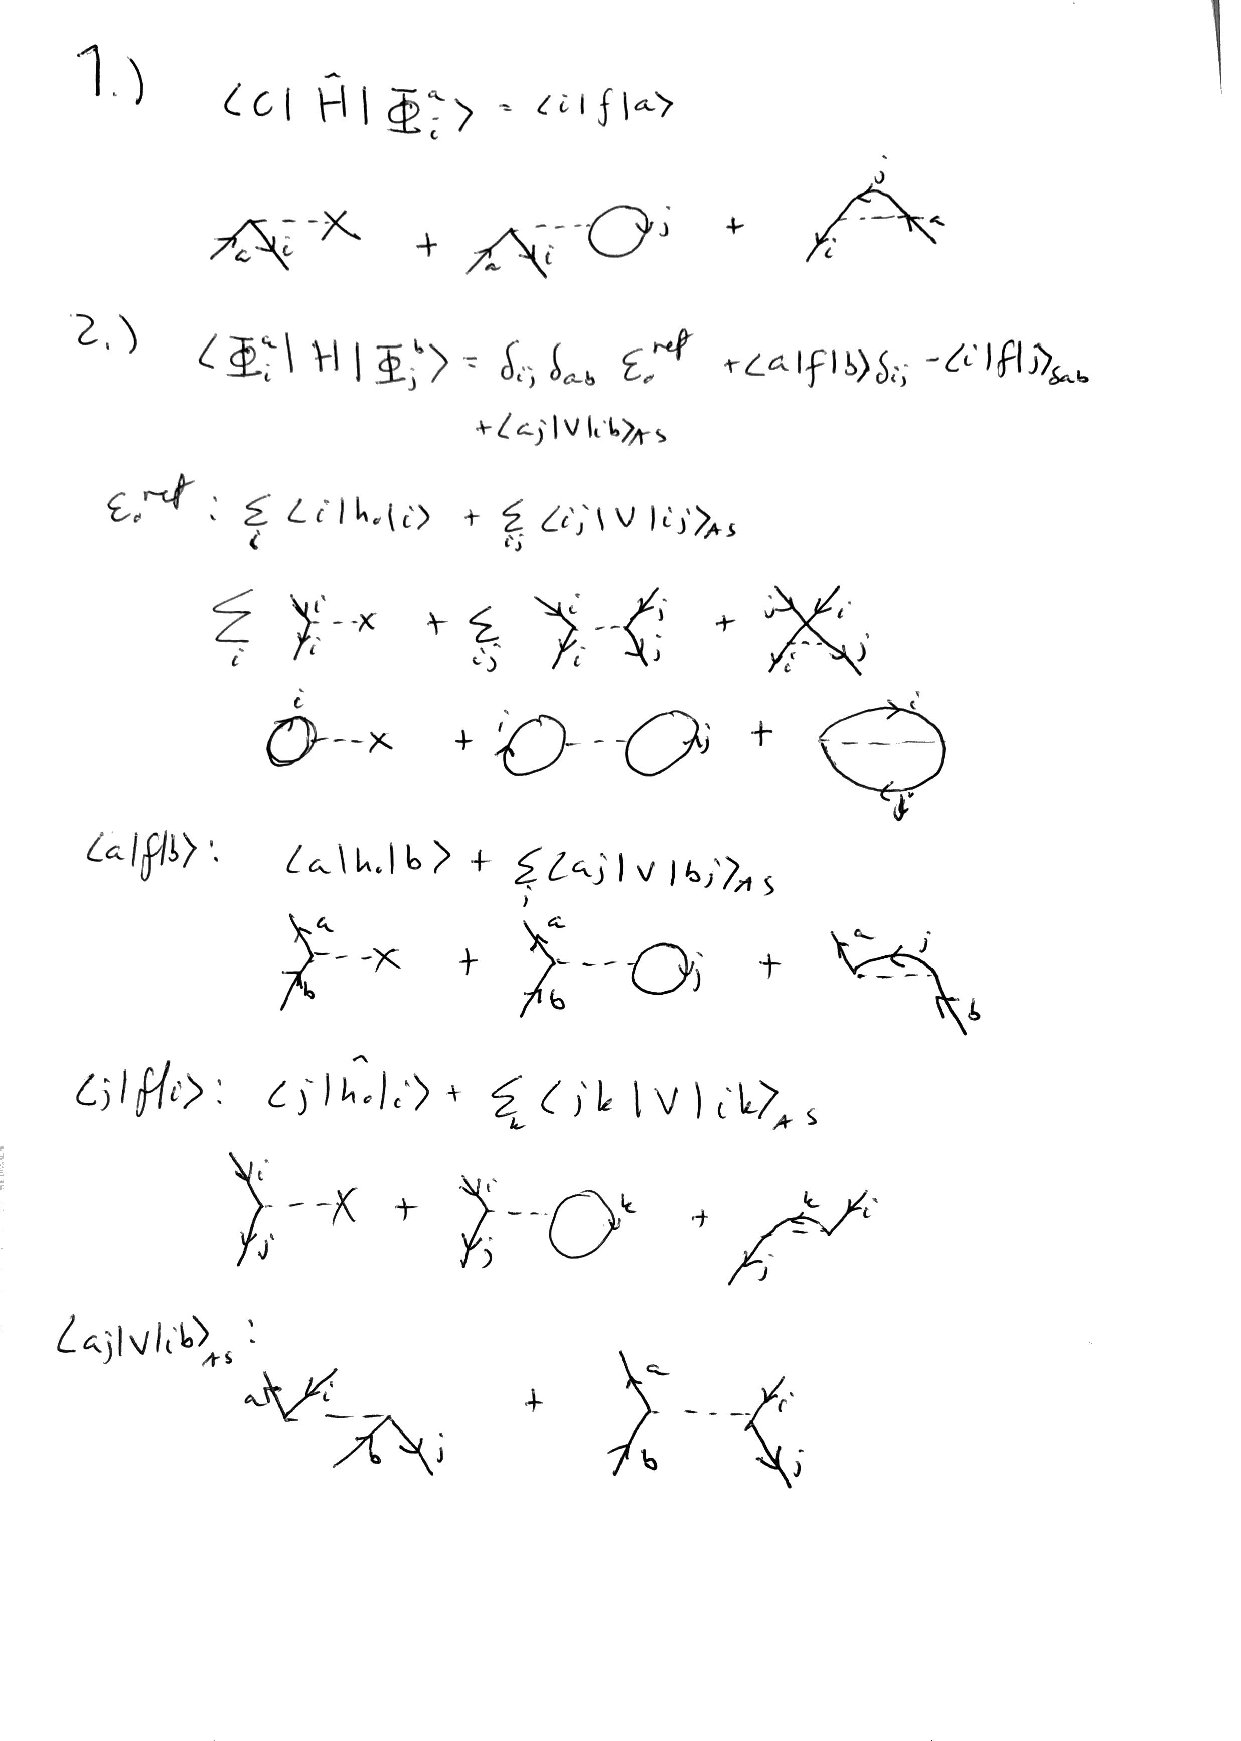
\includepdf[pages=1]{Fys4480mid1.pdf} % First page
\captionof{figure}{1.) is the diagram for $ \bra{ c} \hat{H} \ket{Φ_i^a}$. The diagram for $ \bra{ Φ_i ^a} \hat{ H} \ket{ Φ_j^b}$ is nr.2, and lastly I have the Hartree-Fock diagram nr.3.}
\label{fig:pdf_image_page1}

\newpage
\includepdf[pages=2]{Fys4480mid1.pdf} % Second page
\captionof{figure}{Second page of Fys4480mid1.pdf.}
\label{fig:pdf_image_page2}

\end{document}